\chapter{Referencial Teórico}
\label{ref}
\section{Software Analytics}
\label{ref:sof}
Durante muito tempo a disponibilidade de dados em projetos de software para análise foi um problema. Hoje em dia, com o auxílio da internet, dos projetos de software livre e das características pervasivas e ubíquas da computação, o volume de dados a serem analisados se tornou um problema. Processar e analisar esses dados manualmente se tornou inviável\cite{artAndScience}. Atualmente, por exemplo, pesquisas mostraram que o \textit{Mozilla Firefox} teve 1.3 milhões de relatos de defeitos e outras plataformas como \textit{Sourcefoge.net} e o \textit{Github} hospedam 430.000 e 38 milhões de projetos, respectivamente\cite{informationNeeds}.

Na literatura não existe um consenso da definição de \textit{Software Analytics}, o livro~\cite{artAndScience} por exemplo,  define \textit{Software Analytics} como: "A análise de dados de software para gerentes e engenheiros de software, com o objetivo de capacitar indivíduos e times de desenvolvimento, a ganhar e difundir conhecimento a partir de seus dados para tomar melhores decisões". Essa atividade de análise ajuda a usuários, desenvolvedores e gerentes a responderem questões de introspecção, por exemplo, 'O por que e como um determinado evento ocorreu'. A utilização de \textit{Software Analytics} permite esse tipo de introspecção pois ao invés de propor e considerar a análise de métricas e dados independentemente, ela propõe diferentes tipos de análise em diferentes camadas de documentos, de forma a filtrar, resumir, modelar e realizar experimentações que permitam um melhor entendimento do que está acontecendo dentro do projeto\cite{informationNeeds}.

Hoje é comum empresas como Google, Facebook e Microsoft aplicarem métodos de análise de dados diariamente em seus projetos e produtos. Além disso, o número de conferências interessadas nos assuntos de mineração e análise de artefatos de software cresceu, destacando-se duas, a\textit{Mining Software Repositories} (MSR) e a \textit{PROMISE Conference on Repeatable Experimentes in Software Engineering}. Cada uma possui um foco diferente, sendo a MSR preocupada com a coleta dos dados, enquanto que a PROMISE com a eficácia e repetibilidade da análise de dados.

Diversos autores propõem soluções que utilizam técnicas de \textit{Software Analytics} para ajudar na tomada de decisões em projetos de software. Czerwonka, por exemplo, propôs a plataforma de análise \textit{CODEMINE} depois de observar \textit{inputs}, \textit{outputs} e dados de ferramentas de diversos times na Microsoft. O \textit{CODEMINE} fornece informações de diversos artefatos de software, entre eles: \textit{milestones}, código fonte, \textit{bugtrackers} e outros o que permite que novas pesquisas sejam desenvolvidas neste contexto \protect \cite{softwarePrac}. Já Baysal, propôs a utilização de um \textit{dashboard} como uma ferramenta complementar ao \textit{Bugzilla} para os times de desenvolvimento da Mozilla. Desta forma, os desenvolvedores podiam ter informações mais detalhadas a respeito de \textit{patches}, comentários e \textit{bugs} reportados, auxiliando na tomada de decisões no dia-a-dia \protect \cite{softwarePrac}.

\subsection{Projetos de Software Livre e Software Analytics}
\label{ref:sof:sl}
A análise de dados obtidos de ferramentas de versionamento de código, como o Git, Bazaar, Subversion ou CVS pode trazer informações importantes a respeito da evolução de um projeto de software, por exemplo: o nível de engajamento dos desenvolvedores; o número de defeitos; a qualidade interna do produto; resultados de execução de testes, entre outros\cite{artAndScience}. 

O Github é o maior repositório de software do mundo. Além dos serviços de gerenciamento de código padrões presentes em um sistema baseado em git(\textit{push, commit, pull, clone, fork}), o Github também fornece uma maneira dos desenvolvedores de um projeto interagirem através de \textit{features} de uma rede social. Por exemplo, um desenvolvedor que aprecia um projeto pode marca-lo com uma estrela, de forma que as estrelas de um projeto são um indicador de sua popularidade. Alguns dos projetos mais populares hoje no Github são: JQUERY/JQUERY que é uma biblioteca de \textit{scripting} para HTML, TORVALDS/Linux o projeto do \textit{kernel} do Linux, RAILS/RAILS um framework para a linguagem Ruby e o DOCKER/DOCKER que é um motor de contêineres para aplicações~\cite{githubPop}. 

Devida a alta popularidade do Github, ele é largamente usado para a realização de pesquisas e mineração de dados. Por exemplo, Zho et al. mostra que a adoção de pastas com nomes padrão (\textit{doc, test, examples}) em projetos pode ter um impacto na popularidade do projeto. Já em outro estudo Aggarwal et al. mostra que projetos com uma alta popularidade atraem mais pessoas que queiram contribuir com a \textit{Wiki} e documentação~\cite{githubPop}.

Para que fosse possível a realização destes estudos foi necessário que os repositórios fossem abertos, e que fosse utilizada a API do Github. A API fornecida pelo Github é um ponto de acesso comum por onde é possível extrair informações de repositórios públicos, essas informações podem estar divididas em dois grandes grupos:

\begin{itemize}
    \item \textbf{Metadados:} Os metadados fornecidos são informações associadas a cada \textit{commit} ou \textit{issue}, são: criador(a), data, mensagem do \textit{commit} ou \textit{issue}, a \textit{branch}, o repositório, e o escopo do \textit{commit} ou \textit{issue}. Além disso, na mensagem do \textit{commit} podem haver referencias a outros desenvolvedores, defeitos ou outros \textit{commits} e \textit{issues}.
    \item \textbf{Snapshots:} O código fonte do projeto, que pode ser obtido em diferentes fases do desenvolvimento, já que a ferramente permite que um usuário avance ou retroceda dentro dos \textit{commits}. Desta forma, é possível analisar o código de um projeto referente em vários períodos diferentes.
\end{itemize}

Abaixo, na Figura~\ref{fig:github_api}, podemos ver o digrama de classes da API fornecida pelo Github, com base nesta imagem, é possível ver que as \textit{issues} e informações dos \textit{commiters} são exportadas a partir de um ponto comum de acesso.
\newpage
\begin{figure}[!h]
    \centering
        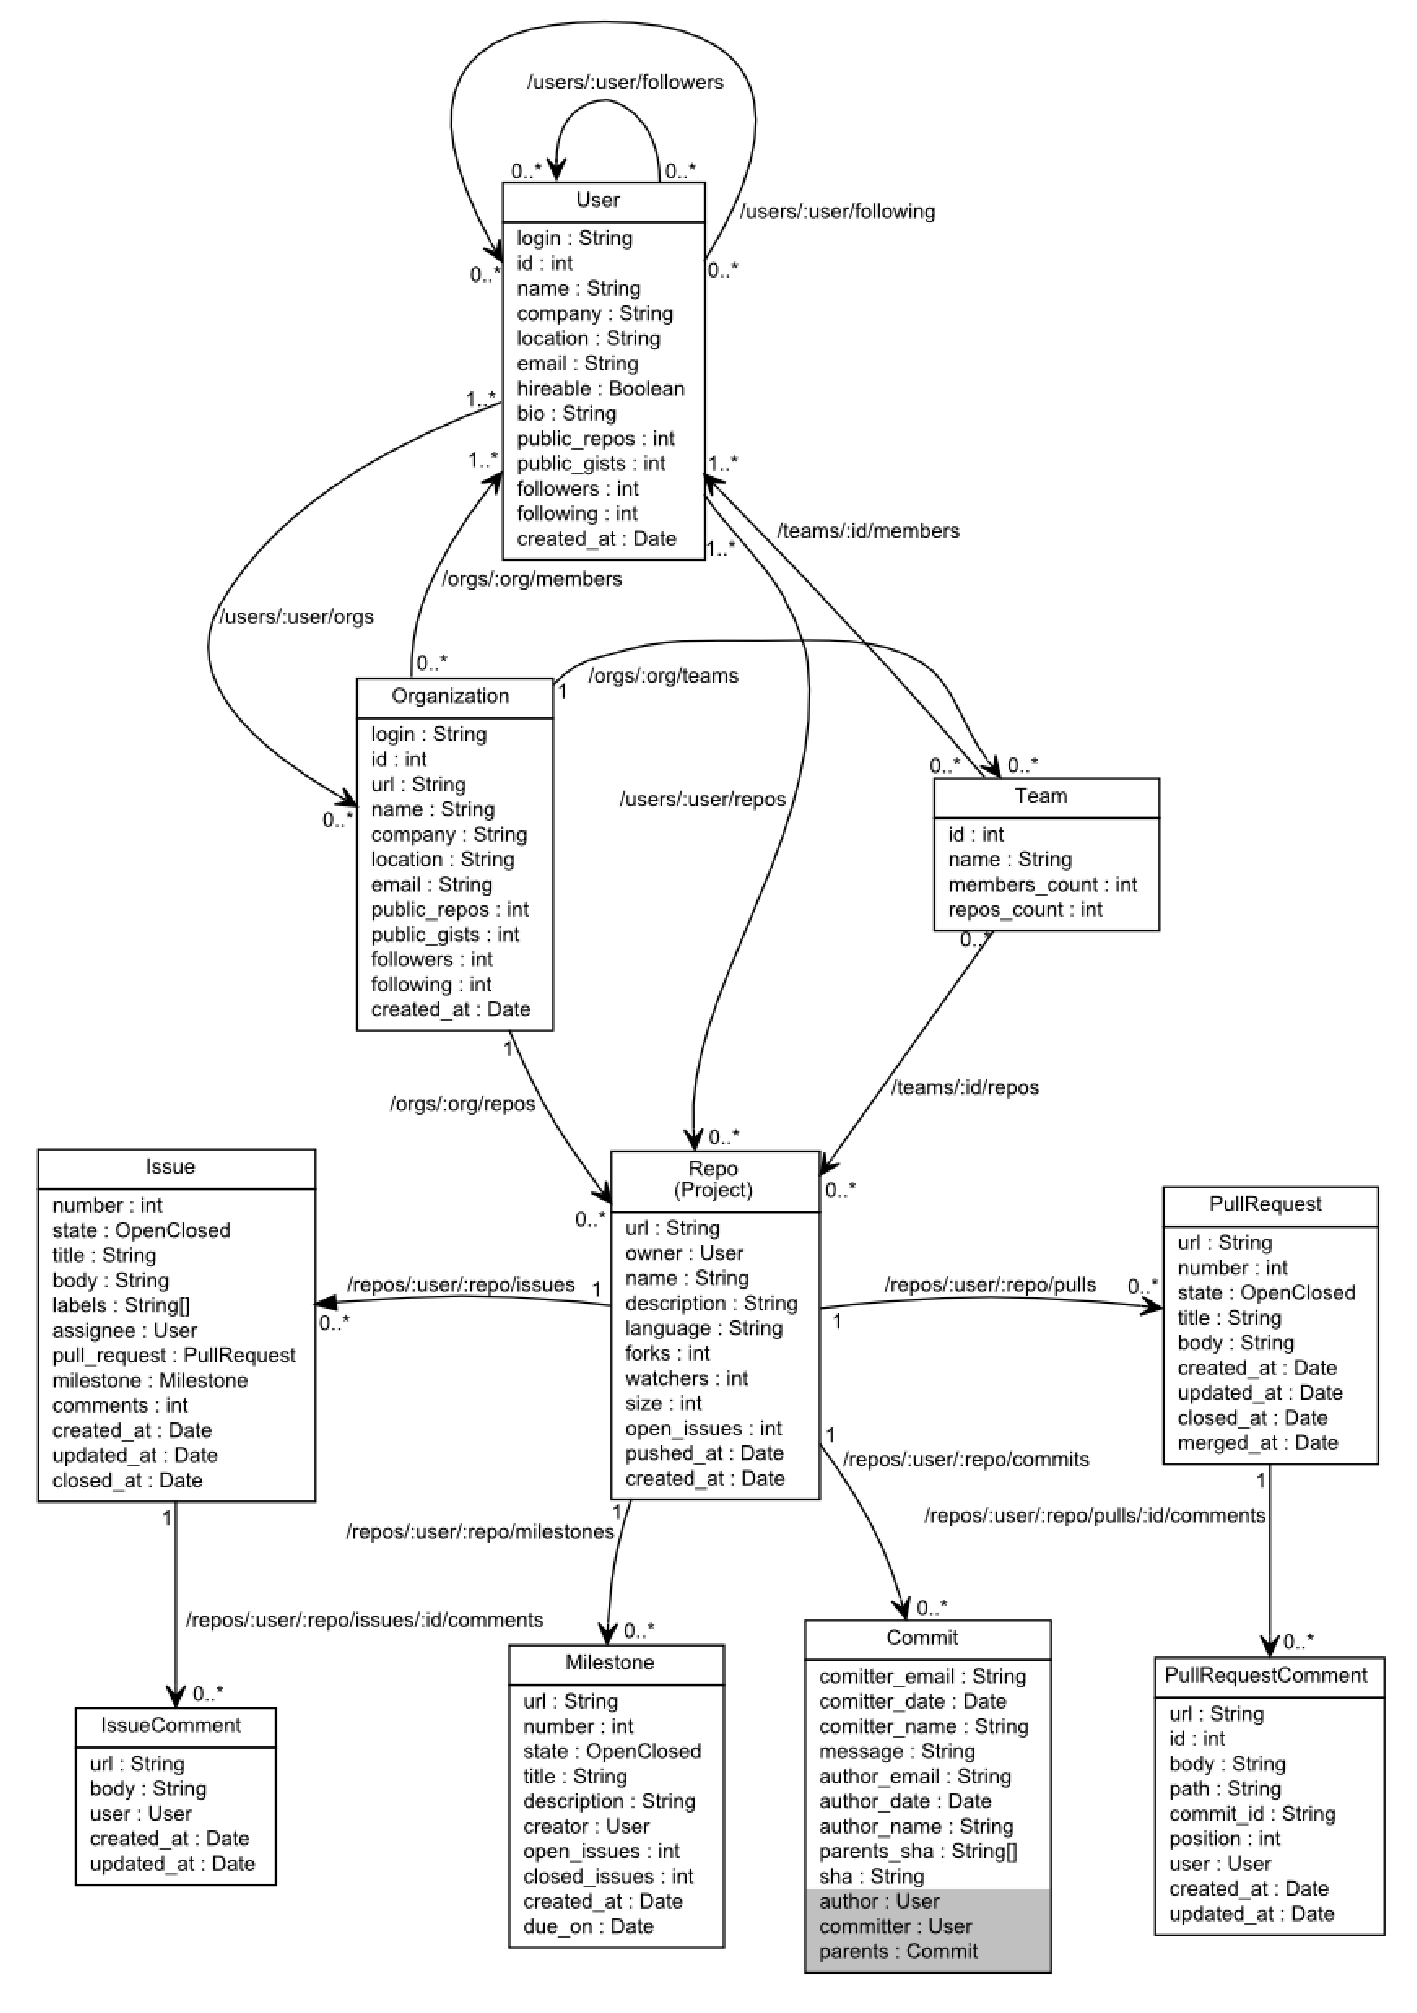
\includegraphics[width=\textwidth,height=\textheight,keepaspectratio=true]{figuras/gtschema.eps}
    \caption{Diagrama do Esquema do Github}
    \label{fig:github_api}
\end{figure}

\section{Centralidade de Redes e o Ranqueamento de Páginas}
\label{ref:cen}
Centralidade é um dos tópicos mais estudados na teoria dos grafos, sendo um tópico de grande importância em estudos de redes sociais~\cite{networks}. Ela determina o grau de importância de um vértice dentre todos os outros dentro de uma rede. Na Figura \ref{fig:centrality} é ilustrado um exemplo de centralidade. O conceito de centralidade de redes já foi aplicado a diversos contextos, dentre eles: investigar a influencia de redes inter organizacionais, estudos de relevância, vantagens em redes de troca, competência em organizações formais, oportunidades de emprego e diversos outros campos do mercado e ciência\cite{centrality}.

\begin{figure}[!h]
    \centering
        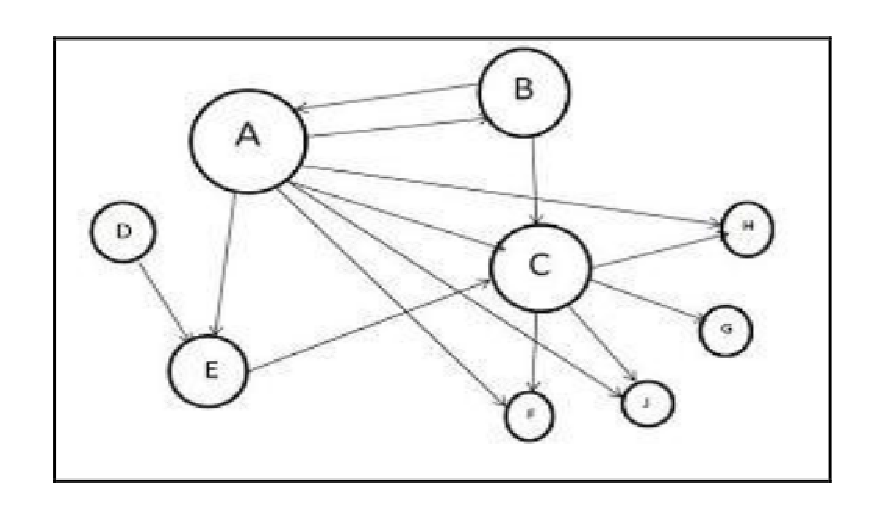
\includegraphics[keepaspectratio=true,scale=0.5]{figuras/centrality.eps}
    \caption{Exemplo de Relevância de um Nó em uma Rede, extraída de \protect \cite{muppidi}.}
    \label{fig:centrality}
\end{figure}

Diversos processos comumente encontrados no dia-a-dia são caracterizados como um processo de fluxo, como por exemplo o envio de e-mails, uma rede social acessada por milhares de usuários e a distribuição de dinheiro e informação entre pessoas. Esses processos diferem em dimensão e tipo, mas ainda assim podem ser comparados e exemplificados. Considerando que os processos de troca de e-mails, troca de informações, uma doença infecciosa que está sendo transmitida em uma população, a distribuição de pacotes e a troca de moedas representam um fluxo, então podemos descrevê-los sob a perspectiva da Teoria dos Grafos\cite{ceflow}. Por exemplo:

\begin{itemize}
\item Dinheiro: Considere uma moeda, ou nota de um dólar, que se move pela economia e muda de mãos a cada transação. Uma nota é indivisível e só pode estar em um lugar em um determinado período de tempo. Na perspectiva da teoria dos grafos, a movimentação de uma nota em uma rede pode ser feita como um \textit{passeio (Walk)}, sendo, desta forma, representado como um processo de Markov~\cite{ceflow}.
\item Fofoca: Imagine uma informação privada que passa por uma rede de empregados de uma empresa. Diferentemente de uma moeda, essa mesma informação pode estar em diversos locais diferentes em um determinado período de tempo, se replicando a cada pessoa que passa a ter acesso a informação, mas geralmente não atravessa o mesmo vértice mais de uma vez, apesar de poder visitar o mesmo nó mais de uma vez. A movimentação desta informação em grafo pode ser representada como uma trilha\footnote{Em um grafo, uma trilha(\textit{trail}) é um passeio (\textit{Walk}) que não possui arestas repetidas}~\cite{ceflow}.
\item E-mail: Um vírus, ou spam de e-mail, que envia mensagens a todos os contatos de uma pessoa simultaneamente pode ser considerado um processo de fluxo. Um e-mail pode ser representado como uma trilha da mesma forma que é realizado com uma informação, já que compartilha propriedades semelhantes, como existir em diversos locais ao mesmo tempo, e geralmente, os e-mails não passam pelo mesmo vértice, ou caminho, duas vezes~\cite{ceflow}.
\item Infecções: O caso de uma infecção em que o hospedeiro ficou imune. A infecção vai passar por duplicação de pessoa a pessoa, mas nunca vai voltar a infectar aqueles que já se tornaram imunes~\cite{ceflow}.
\item Pacotes: Um pacote de rede tem a característica de possuir um remetente e um destinatário. Normalmente é preferível que o pacote percorra o menor caminho possível até chegar ao seu destino. Dessa forma, a movimentação do pacote deve seguir o caminho geodésico\footnote{Um caminho geodésico em um grafo é composto pelas arestas que representam o menor caminho entre dois vértices.} pela rede de roteadores~\cite{ceflow}. 
\end{itemize}

A partir destas ideias discutidas a respeito de centralidade, pretende-se modelar as \textit{issues} de um repositório de código como um processo de fluxo. Uma \textit{issue} em repositório é uma informação única que pode ser associada a outras \textit{issues}, pessoas ou trechos específicos de código. Sendo assim, as informações contidas em \textit{issue} se mantem a mesma, porém com a característica de poder influenciar o planejamento e o desenvolvimento do projeto.

Ao longo dos anos, diferentes métodos de medida de centralidade foram criados, entre eles: Centralidade de Grau, Proximidade \textit{(Closeness)}, Intermediação \textit{(Betweenness)}, Autovetor \textit{(Eigen Vector)}, Informação, Intermediação de Fluxo, \textit{Rush Index}, Medidas de Influencia de Katz, Hubbell, Hoede e Taylor~\cite{centrality}. Estes métodos diferem nas suposições iniciais que fazem para alcançar o objetivo de determinar o nó com maior importância, por exemplo, o algoritmo de Freeman de proximidade e intermediação conta apenas os caminhos geodésicos entre os nós, assumindo que qualquer fluxo que percorra uma rede, siga sempre pelo caminho mais curto. Outros algoritmos como a centralidade de autovetor de Bonacich conta travessias, o que assume que as trajetórias podem ser sinuosas, atravessando nós e arestas repetidas vezes até chegar ao destino~\cite{Bonacich87}.

A partir de todos estes métodos discutidos por~\cite{centrality} e \protect \cite{Bonacich87}, foi escolhido um algoritmo para ser aplicado no exemplo de uso realizado nesta primeira etapa da monografia. O algoritmo escolhido foi o \textit{Page Ranking}, ou algoritmo de ranqueamento de paginas, a escolha deste algoritmo deu-se ao fato de ser um dos algoritmos mais utilizados no calculo de relevância e ser largamente estudado \cite{brin}, o que inclui pesquisas como a realizada por \cite{muppidi} que realiza uma comparação entre os algoritmos de ranqueamento contemporâneos. A próxima seção deste capítulo apresenta a fundamentação teórica a respeito do algoritmo de ranqueamento de páginas

\subsection{Ranqueamento de Páginas}
\label{ref:cen:pag}
O algoritmo de ranqueamento de páginas foi criado por Larry Page e Sergey em 1996. Ele permite calcular a importância relativa de páginas da web e tem aplicações em mecanismos de busca, estimativas de trafego e navegação na web. O algoritmo foi criado com o intuito de prover uma solução de busca de informações na web a partir da estrutura dos links, usada no hipertexto da web. \cite{pageRank}.

A premissa do algoritmo de ranqueamento de páginas é que cada página na web possui um número de \textit{links} de saída e de entrada, e que páginas com um grande número de \textit{links} são mais importantes do que as com poucos \textit{links}. Além disso, o algoritmo também leva em consideração a relevância dos \textit{links} de entrada de uma página, ou seja, se uma página da web possui um \textit{link} de entrada que possui uma alta relevância, essa página tende a ser mais importante que outra que possua vários \textit{links} mas que vieram de páginas menos relevantes.

A função de ranqueamento de páginas é uma função recursiva definida na seguinte forma:

Seja $x$ uma página da web. Então:
\begin{itemize}
    \item $PR(x)$ \textit{Page rank} da página  $x$
    \item $PR(y)$ \textit{Page rank} da página  $y$
    \item $L(x)$ é o conjunto de páginas que possuem link para $x$
    \item $C(y)$ é o grau de saída de $y$
    \item $\alpha$ é a probabilidade de um pulo aleatório
    \item $N$ é o número total de web-sites
\end{itemize}
\[\displaystyle PR(x) := \alpha \left ( \frac{1}{N} \right ) + (1-\alpha) \sum_{y\in L(x)} \frac{PR(y)}{C(y)}\]

A função de ranqueamento de páginas não ranqueia um \textit{web-site} por completo, mas páginas individuais de cada \textit{web-site}. O \textit{page rank} de uma página $y$ que possui \textit{links} para $x$ também não influencia o \textit{page rank} de $x$ uniformemente. No algoritmo de ranqueamento de páginas o \textit{page rank} de uma página $y$ é balanceado com base no grau de saída~\footnote{O grau de saída de um vértice em um grafo direcionado é igual ao número de caudas (\textit{tails}) incidentes ao vértice.} $C(y)$ na página $y$, de forma que quanto maior o número de \textit{links} de saída da página $y$ menos a página $x$ vai se beneficiar disto. Depois deste passo, é realizado o somatório do \textit{page rank} das páginas $y$, desta forma, cada link de entrada para a página $x$ aumenta seu \textit{page rank}~\cite{pageRank}.

Depois deste primeiro passo, a soma do \textit{page rank} $PR(y)$ é multiplicada por um fator de amortecimento $\alpha$. Este fator representa a probabilidade de um pulo aleatório em uma determinada página, ou seja, a probabilidade de que uma pessoa que esteja surfando na \textit{web}, e esteja em uma pagina $y$ clique em qualquer um dos \textit{links} desta página. A probabilidade de que uma pessoa clique em um dos \textit{links} de uma página é puramente baseada no número de \textit{links} da página, e a probabilidade que ela chegue em uma página específica é a soma das probabilidades de cada \textit{link} que a pessoa teve que seguir para chegar a ela. Por se tratar de uma probabilidade, o $\alpha$ assume valores entre 0 e 1, porém para muitos casos é sugerido o uso de 0.85~\cite{pageRank}. 

Na Figura~\ref{fig:page_rank} é apresentado um exemplo como a relevância de uma página influencia as páginas seguintes.

\begin{figure}[!h]
    \centering
        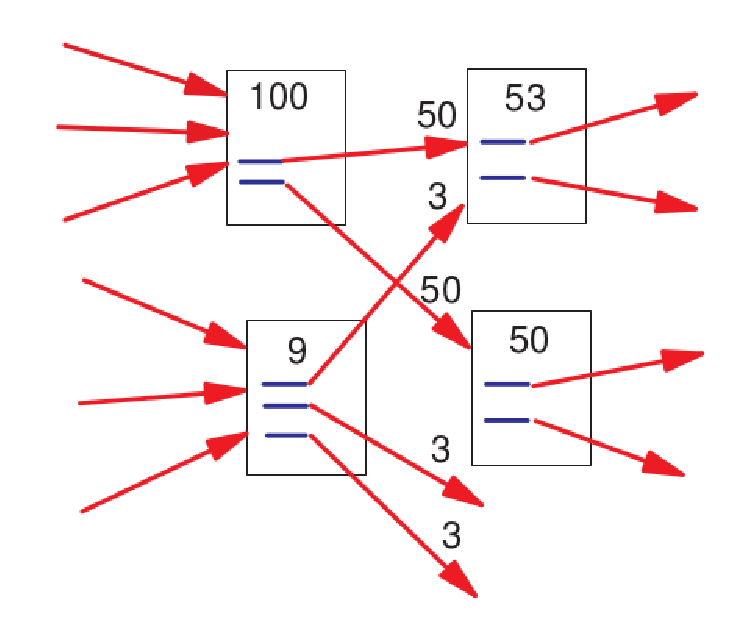
\includegraphics[keepaspectratio=true,scale=0.5]{figuras/page_rank.eps}
    \caption{Simplificação do Cálculo de Ranqueamento de Páginas, extraída de \protect \cite{pageRank}.}
    \label{fig:page_rank}
\end{figure}

\begin{figure}[!h]
    \centering
        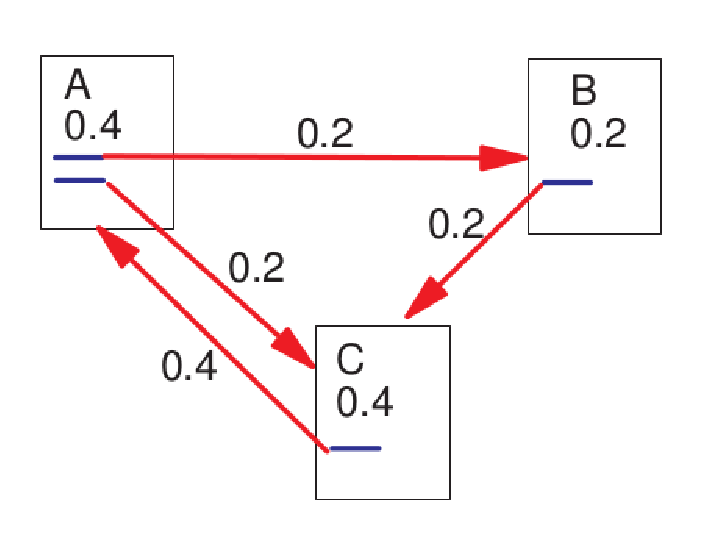
\includegraphics[keepaspectratio=true,scale=0.5]{figuras/page_rank2.eps}
    \caption{Simplificação do Cálculo de Ranqueamento de Páginas, extraída de \protect \cite{pageRank}.}
    \label{fig:page_rank2}
\end{figure}

A Figura~\ref{fig:page_rank} ilustra como o ranqueamento de páginas se divide através das paginas e como ele contribui para o ranque das páginas seguintes. Na Figura~\ref{fig:page_rank} é possível ver como uma página que possui um \textit{page rank} acumulado de 100 distribui seu ranque igualmente para as paginas seguintes, de forma que cada um dos seus dois \textit{links} receba 50 de ranque. Já em umá página que possui 9 de ranque acumulado, distribui igualmente 3 de ranque para cada um dos seus 3 \textit{links} subsequentes. Na Figura~\ref{fig:page_rank2} é ilustrado como um estado estável pode ser alcançado depois que o algoritmo é executado em um conjunto de páginas, de forma que o ranque de uma página seja distribuído igualmente para as páginas posteriores a ela. 

\begin{figure}[!h]
    \centering
        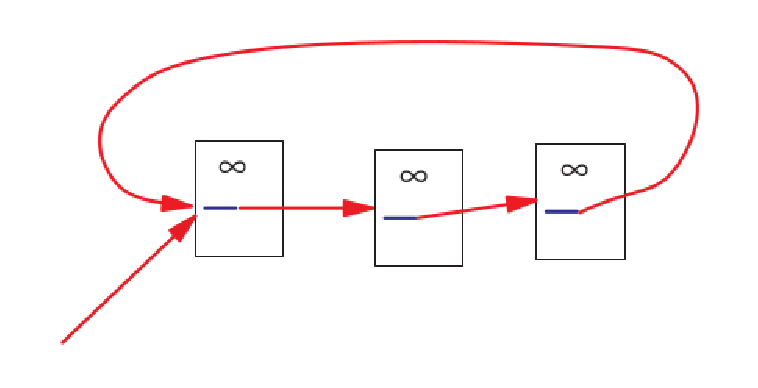
\includegraphics[keepaspectratio=true,scale=0.5]{figuras/page_rank3.eps}
    \caption{\textit{Loop} de Ranqueamento, extraída de \protect \cite{pageRank}.}
    \label{fig:page_rank3}
\end{figure}

Um dos problemas dessa função de ranqueamento, é que caso duas páginas da web que apontem uma para outra, e uma terceira aponte para qualquer uma destas, o \textit{loop} vai acumular ranque porém, nunca vai distribuir isso para nenhuma outra página seguinte. Na ilustração apresentada na Figura~\ref{fig:page_rank3}, possível observar esse fenômeno.

\section{Considerações Finais do Capítulo}
Neste capítulo foi apresentado o referencial teórico a respeito dos tópicos de \textit{Software Analytics}, Centralidade e o algoritmo \textit{Page Ranking}. No próximo capítulo é apresentada a metodologia utilizada neste estudo, passando primeiramente pela definição da população de estudo, depois as técnicas de intervenção que devem ser aplicadas e, finalmente, como a análise dos dados deve ser feita ao final desta primeira etapa da monografia.
